\chapter{Introduction}
\label{ch:introduction}

In this chapter the two goals of this thesis are discussed.
The fist goal is to automate releasing a system to multiple platforms.
The second goal is to integrate different test configurations of a software system into a set of test environments.



\section{Release automation}
\label{sec:introduction:release-automation}

The software company Dynatrace\footnote{\url{https://www.dynatrace.com/}} is offers two products called OneAgent and ActiveGate.
Both products are also available in a containerized format.
Using this containerized format, it is possible to run them in computer clusters managed by software such as Kubernetes\footnote{\url{https://kubernetes.io/}}.

However, in order to run correctly, applying some cluster specific configuration is necessary.
These configurations are mostly provided using files in the YAML format\cite{UnderstandingKubernetesObjects}.
Before applying these configurations, they have to be created and edited by a customer to fit their environment.

In order to remove the necessity of complicated configurations and possibility of human error, Dynatrace maintains the Dynatrace Operator (DTO).
The DTO is an open-source project, which can be deployed on a computer cluster.
After deployment, it allows applying a special configuration file, which contains all needed configuration options a customer must or can apply to either a OneAgent or ActiveGate deployment.
It then automatically manages the deployment of these products and their lifecycle.

This operator\cite{OperatorPattern} is released, in the form of deployment files to a variety of platforms.
These platforms, at the time of writing, are
its GitHub\footnote{\url{https://github.com/}} repository\footnote{\url{https://github.com/Dynatrace/dynatrace-operator}},
the RedHat Container Catalog\footnote{\url{https://catalog.redhat.com/}},
the Community Operators repository\footnote{\url{https://github.com/operator-framework/community-operators}},
the ArtifactHub\footnote{\url{https://artifacthub.io/}} of Helm\footnote{\url{https://helm.sh/}},
the Rancher\footnote{\url{https://rancher.com/}} repository\footnote{\url{https://github.com/rancher/helm3-charts}} for Helm charts and
the Google Kubernetes Engine\footnote{\url{https://cloud.google.com/kubernetes-engine}} (GKE) Marketplace\footnote{\url{https://cloud.google.com/marketplace}}.

The releases to all of these platforms are currently done manually.
Since every platform has its own special handling of a release, every DTO release takes a lot of time.
The work time needed for a single release is between four workdays and one and a half workweeks, as seen in figure\ \ref{fig:introduction:time-spent}.

\begin{figure}
    \label{fig:introduction:time-spent}
    \centering
    \begin{minipage}{0.45\textwidth}
        \centering
        
\includegraphics[width=0.9\textwidth]{img/introduction/lower_end}
        \caption{Lower end of the time needed to publish a release}
        \label{fig:introduction:lower-end}
    \end{minipage}\hfill
    \begin{minipage}{0.45\textwidth}
        \centering
        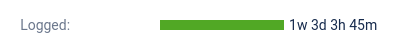
\includegraphics[width=0.9\textwidth]{img/introduction/upper_end}
        \caption{Upper end of the time needed to publish a release}
        \label{fig:introduction:upper-end}
    \end{minipage}
\end{figure}

Therefore, the first of two goals of this thesis is to automate as much of the release process as possible.
In order to automate this process, a system is needed, which executes all, or at least most of, the actions that are currently done by a human.
Such a system may take the form of a so-called continuous integration (CI) / continuous deliver (CD)  pipeline.

A CI/CD pipeline is a defined series of actions, which are automatically executed\cite{WhatIsACiCdPipeline}.
The goal of such a pipeline is to do a combination, or all, of building, testing, packaging and releasing a software product\cite{WhatIsACiCdPipeline}.
In this case, Concourse\footnote{\url{https://concourse-ci.org/}} is used as a base of the system of this paper.
A pipeline will be created, with the purpose of automatically preparing a release of the DTO, leaving, at best, a single push of a button to do for a human.

\section{Test configuration integration}
\label{sec:introduction:test-configuration-integration}

In order to deliver the DTO to customers in a reliable state, it undergoes a series of End-to-End (E2E) tests.
Until now, these tests have been manually created and ran with previously defined configurations.
A configuration here describes a set of input variables for the DTO, defined in the YAML format.

While the amount of tests is currently not a problem, the amount of configurations is.
The number of configurations has grown considerably during its development.
So much so, that neither manually defining all configurations, nor testing all of them is practicably doable.
Mitigating this problem is the second goal of this thesis's system.

The aim is to create a user interface.
This user-interface must allow a Dynatrace employee to create apply a configuration to a pipeline running E2E tests.
Preferably implemented as a web application.

This subsystem must be able to do at least three things.
First, it must be possible to create and apply a randomized configuration based on predefined values.
Secondly, it must be possible to create and apply a manually selected configuration, for example, to allow an employee to recreate a previously failing scenarion.
Finally, it must be possible to create and manage the configuration and predefine values accordingly.



